\documentclass{article}

\usepackage{ulem}
\usepackage{mathrsfs}

\usepackage{indentfirst}
\setlength{\parindent}{2em}
\usepackage{listings}
\usepackage[usenames,dvipsnames]{xcolor}

\usepackage{graphicx}
\usepackage{subfigure}


\usepackage{amsmath}

%超链接
\usepackage{hyperref}
\hypersetup{
	bookmarks=true,
	colorlinks=true,
	linkcolor=black
	}



\definecolor{mygreen}{rgb}{0,0.6,0}
\definecolor{mygray}{rgb}{0.5,0.5,0.5}
\definecolor{mymauve}{rgb}{0.58,0,0.82}
\lstset{
 backgroundcolor=\color{lightgray}, 
 basicstyle = \footnotesize,       
 breakatwhitespace = false,        
 breaklines = true,                 
 captionpos = b,                    
 commentstyle = \color{mygreen}\bfseries,
 extendedchars = false,             
 frame =shadowbox, 
 framerule=0.5pt,
 keepspaces=true,
 keywordstyle=\color{blue}\bfseries, % keyword style
 language = C++,                     % the language of code
 otherkeywords={string}, 
 numbers=left, 
 numbersep=5pt,
 numberstyle=\tiny\color{mygray},
 rulecolor=\color{black},         
 showspaces=false,  
 showstringspaces=false, 
 showtabs=false,    
 stepnumber=1,         
 stringstyle=\color{mymauve},        % string literal style
 tabsize=2,          
 title=\lstname                      
}





\title{The Third Week Report}
\author{Lu Guorui}
\date{2018.6.10}
\usepackage[a6paper,left=10mm,right=10mm,top=15mm,bottom=15mm]{geometry}

\begin{document}
\maketitle
\tableofcontents

\newpage


\addcontentsline{toc}{section}{Python Learning}
\section*{Python Learning}

\section{Complier}
\subsection{Pycharm}
The installation of Pycharm is relatively simple. Just be aware of the following points:
\begin{itemize}
\item Make sure you have installed pip3.
\item Make sure your have set interpreter to python3.5
\item There is no numpy when Pycharm is downloaded from official website, you should add it in "$Settings -> Project -> Project interpreter$". 
\end{itemize}

\subsection{Vim}
Although Pycharm is powerful, I prefer the vim's concision and efficiency. But you are supposed to configure all the functions by yourself.

\subsubsection{The steps of configuring vim \protect\footnotemark[1]}

\footnotetext[1]{Main Source:
\begin{enumerate}
\item https://blog.csdn.net/u012450329/article/details/52539058
\item https://blog.csdn.net/hang916/article/details/79652645
\end{enumerate}
}

\begin{enumerate}


\item Make sure the catalog, \textbf{~/.vim/bundle}, exist. If not, creat a new one.

\item Install the Vundle:

\begin{itemize}
\item \textnormal{The old version:} \bf {git clone https://github.com/gmarik/Vundle.vim.git ~/.vim/bundle/Vundle.vim}
\item \textnormal{The new version:} \bf {git clone https://github.com/VundleVim/Vundle.vim.git ~/.vim/bundle/Vundle.vim}
\end{itemize}
I used the old version.


\item New the \textbf{.vimrc} file


\item Add the following contents in your new file:
\begin{lstlisting}
set nocompatible              " required
filetype off                  " required

" set the runtime path to include Vundle and initialize
set rtp+=~/.vim/bundle/Vundle.vim
call vundle#begin()

" alternatively, pass a path where Vundle should install plugins
" call vundle#begin('~/some/path/here')

" let Vundle manage Vundle, required
Plugin 'gmarik/Vundle.vim'
Plugin 'vim-scripts/indentpython.vim'
Plugin 'tmhedberg/SimpylFold'
"Plugin 'aralla/completor.vim'
Plugin 'scrooloose/syntastic'
Plugin 'nvie/vim-flake8'
Plugin 'jnurmine/Zenburn'
Plugin 'altercation/vim-colors-solarized'


Plugin 'tell-k/vim-autopep8'


Plugin 'scrooloose/nerdtree'

Plugin 'Xuyuanp/nerdtree-git-plugin'

"Plugin 'Lokaltog/vim-powerline'Valloric/YouCompleteMe'
"Plugin 'maralla/completor.vim'
"Plugin 'scrooloose/syntastic'
"Plugin 'nvie/vim-flake8'
"Plugin 'jnurmine/Zenburn'
"Plugin 'altercation/vim-colors-solarized'

"Plugin 'scrooloose/nerdtree'

"Plugin 'Xuyuanp/nerdtree-git-plugin'

"Plugin 'Lokaltog/vim-powerline'

Plugin 'Yggdroot/indentLine'


Plugin 'kien/ctrlp.vim'

Plugin 'jiangmiao/auto-pairs'



" Add all your plugins here (note older versions of Vundle used Bundle instead of Plugin)

" All of your Plugins must be added before the following line
call vundle#end()            " required

filetype plugin indent on    " required

let g:completor_python_binary = '/usr/bin/python3.5'
let Tlist_Auto_Highlight_Tag=1
let Tlist_Auto_Open=1
let Tlist_Auto_Update=1
let Tlist_Display_Tag_Scope=1
let Tlist_Exit_OnlyWindow=1
let Tlist_Enable_Dold_Column=1
let Tlist_File_Fold_Auto_Close=1
let Tlist_Show_One_File=1
let Tlist_Use_Right_Window=1
let Tlist_Use_SingleClick=1
nnoremap <silent> <F8> :TlistToggle<CR>

filetype plugin on
autocmd FileType python set omnifunc=pythoncomplete#Complete
autocmd FileType javascrīpt set omnifunc=javascriptcomplete#CompleteJS
autocmd FileType html set omnifunc=htmlcomplete#CompleteTags
autocmd FileType css set omnifunc=csscomplete#CompleteCSS
autocmd FileType xml set omnifunc=xmlcomplete#CompleteTags
autocmd FileType php set omnifunc=phpcomplete#CompletePHP
autocmd FileType c set omnifunc=ccomplete#Complete

let g:pydiction_location='~/.vim/tools/pydiction/complete-dict'
set autoindent
set expandtab
set tabstop=4
set shiftwidth=4
set number
set lines=35 columns=118


set number "显示行号
set nowrap    "不自动折行
set showmatch    "显示匹配的括号
set scrolloff=3        "距离顶部和底部3行"
set encoding=utf-8  "编码
set fenc=utf-8      "编码
set mouse=v        "启用鼠标
set hlsearch        "搜索高亮

let python_highlight_all=1
syntax on    "语法高亮


hi BadWhitespace guifg=gray guibg=red ctermfg=gray ctermbg=red
au BufRead,BufNewFile *.py,*.pyw,*.c,*.h
\ set tabstop=4   "tab宽度
\ set softtabstop=4
\ set shiftwidth=4
\ set textwidth=79  "行最大宽度
"\ set expandtab       "tab替换为空格键
\ set autoindent      "自动缩进
\ set fileformat=unix  "保存文件格式


map <F5> :call RunPython()<CR>
func! RunPython()
    exec "W"
    if &filetype == 'python'
    ¦   exec "!time python2.7 %"
    endif
endfunc

"split navigations
nnoremap <C-J> <C-W><C-J>
nnoremap <C-K> <C-W><C-K>
nnoremap <C-L> <C-W><C-L>
nnoremap <C-H> <C-W><C-H>

set foldmethod=indent
set foldlevel=99

let g:SimpylFold_docstring_preview=1



au BufNewFile,BufRead *.js, *.html, *.css
\ set tabstop=2
\ set softtabstop=2
\ set shiftwidth=2


au BufRead,BufNewFile *.py,*.pyw,*.c,*.h match BadWhitespace /\s\+$/


"python with virtualenv support
"py << EOF
"import os
"import sys
"if 'VIRTUAL_ENV' in os.environ:
"  project_base_dir = os.environ['VIRTUAL_ENV']
"  activate_this = os.path.join(project_base_dir, 'bin/activate_this.py')
"  execfile(activate_this, dict(__file__=activate_this))
"EOF


if has('gui_running')
  set background=dark
  colorscheme solarized
else
  colorscheme zenburn
endif

map <C-n> :NERDTreeToggle<CR>

hi MatchParen ctermbg=DarkRed guibg=lightblue


autocmd FileType python noremap <buffer> <F7> :call Autopep8()<CR>


map <F8> :call FormartSrc()<CR>

"定义FormartSrc()
func FormartSrc()
exec "w"
if &filetype == 'c'
exec "!astyle --style=ansi --one-line=keep-statements -a --suffix=none %"
elseif &filetype == 'cpp' || &filetype == 'hpp'
exec "r !astyle --style=ansi --one-line=keep-statements -a --suffix=none %> /dev/null 2>&1"
elseif &filetype == 'perl'
exec "!astyle --style=gnu --suffix=none %"
elseif &filetype == 'py'||&filetype == 'python'
exec "r !autopep8 -i --aggressive %"
elseif &filetype == 'java'
exec "!astyle --style=java --suffix=none %"
elseif &filetype == 'jsp'
exec "!astyle --style=gnu --suffix=none %"
elseif &filetype == 'xml'
exec "!astyle --style=gnu --suffix=none %"
endif
exec "e! %"
endfunc
"结束定义FormartSrc
\end{lstlisting}


\item After step4, my vim gives an error whic is roughly said that it can't find the Zenburn. So we should copy the folder from \textbf{~/.vim/bundle} \textnormal{to} \textbf{/usr/share/vim/vim74/}.

\item Then you can open the vim and input:"\textbf{:PluginInstall}". But this command failed on my computer. Unfortunately, there is no method that can solve my problem, and yet I found a command "\textbf{vim +PluginInstall +qall}" has the same effect as "\textbf{:PluginInstall}" in vim. What's more, I saw what the log of errors said was "\textbf{Permission denied}", so tried to input "\textbf{sudo vim +PluginInstall +qall}" and succeed.


\end{enumerate}


Let's have a look of what my vim looks like after configuration through the figure \ref{my vim}:
\begin{figure}[htbp]
\centering
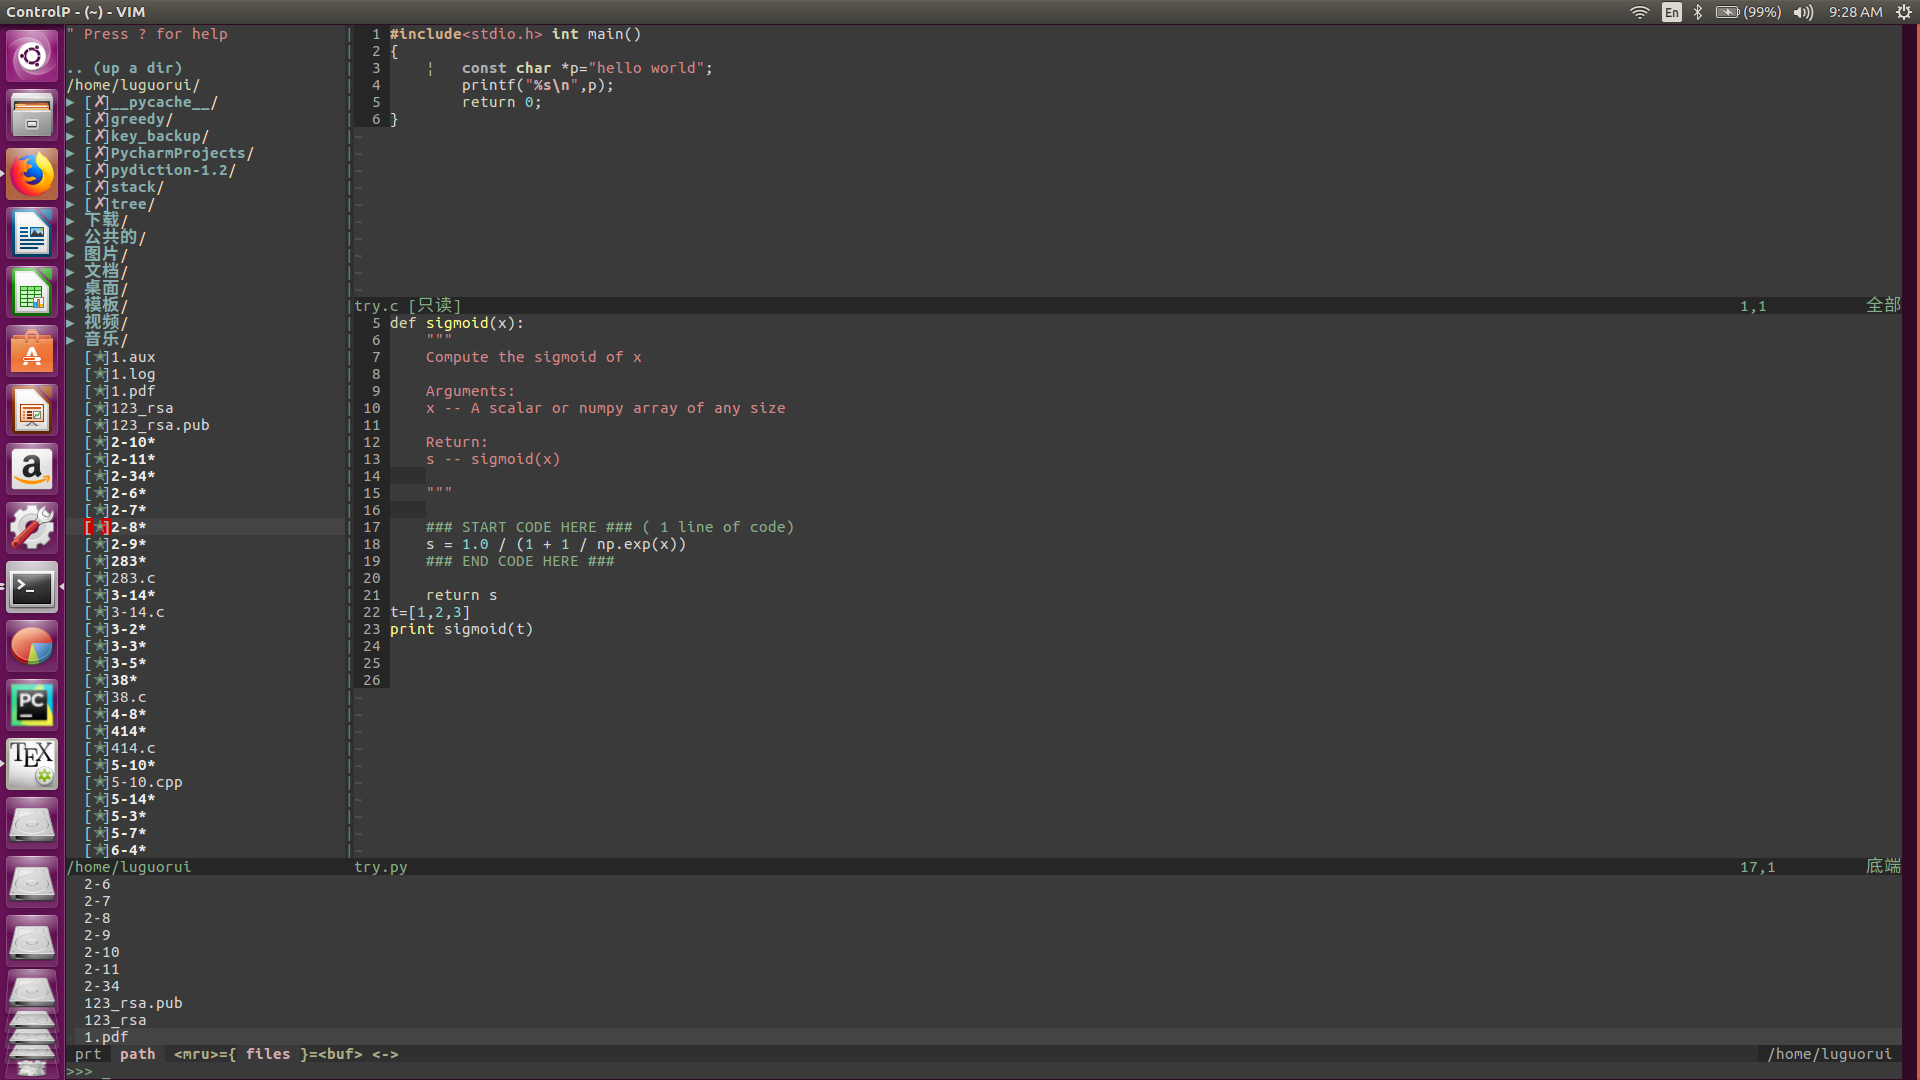
\includegraphics[width=9cm]{2018-06-09 09-28-03屏幕截图.png}
\caption{My Vim}
\label{my vim}
\end{figure}

\addcontentsline{toc}{section}{Practical aspects of DeepLearning}
\section*{Practical aspects of DeepLearning}
\setcounter{section}{0}
\section{Normalizing inputs}

\subsection{Explanation} 
 The essence of normalization is a kind of linear transformation which compresses and parallel moves the data. Linear transformation has many good properties, one of which is that it won't change the relative order of data. These properties ensure our data won't be invalidated while we transform them. \par
We can also have a intuitive view of normalization from geometrical point of view. Let's look at the pictures below.

\begin{figure}[htbp]
\begin{minipage}[t]{0.45\linewidth}
\centering
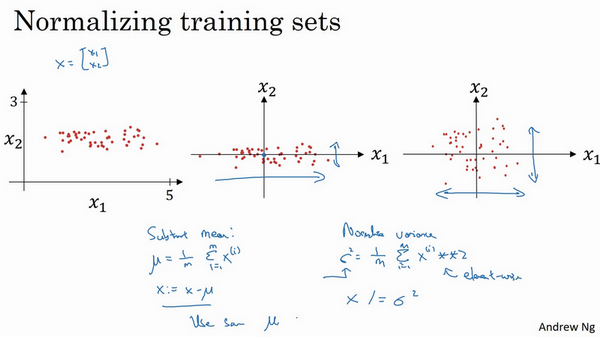
\includegraphics[width=5cm]{normalization_data.png}
\caption{Data}
\end{minipage}
\hfill
\begin{minipage}[t]{0.45\linewidth}
\centering
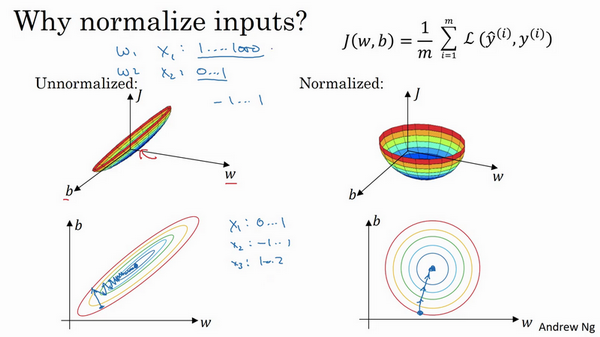
\includegraphics[width=5cm]{normalization_J_function.png}
\caption{Const function}
\label{J}
\end{minipage}
\end{figure}

Obviously, normalization makes data more concentrated.
\subsection{Steps of normalizing inputs}
\begin{enumerate}

\item $\mu = \frac{1}{m}\sum\limits_{i =1}^{m}x^{(i)}$
\item $\sigma^{2}= \frac{1}{m}\sum\limits_{i =1}^{m}{({x^{(i)})}^{2}}$

\end{enumerate}

As once the data has been determined, $\mu$ and $\sigma$ are both constants , so it can be seen as linear transformation, which can makes the process more efficient.

\section{Mini-batch gradient descent}
We can divided our training set into many smaller mini-bitch while training the neural network, which can makes the process more efficienct.\par
Mini-batch gradient descent allows our neural network carry out more gradient decents while it can only count one gradient descent if we don't use mini-batch. Considering the way that computer store, we usually set the  mini-batch's size to be an integer multiple of 2. 



\addcontentsline{toc}{section}{Some thoughts from SeetaTech's vedios}
\section*{Some thoughts from SeetaTech's videos}
Apart from deeplearning.ai, I also watched some videos produced by SeetaTech, which gave me a deeper understanding.
\setcounter{section}{0}
\section{How can we see an object}
There are many nerve cells in our brains. From the experiment in figure  \ref{experiment} we can know that each of them speciallized in judging a specific condition and transmit the information to the cell which judges a more complex condition.
 
\begin{figure}[htbp]

\begin{minipage}[t]{0.45\linewidth}
\centering
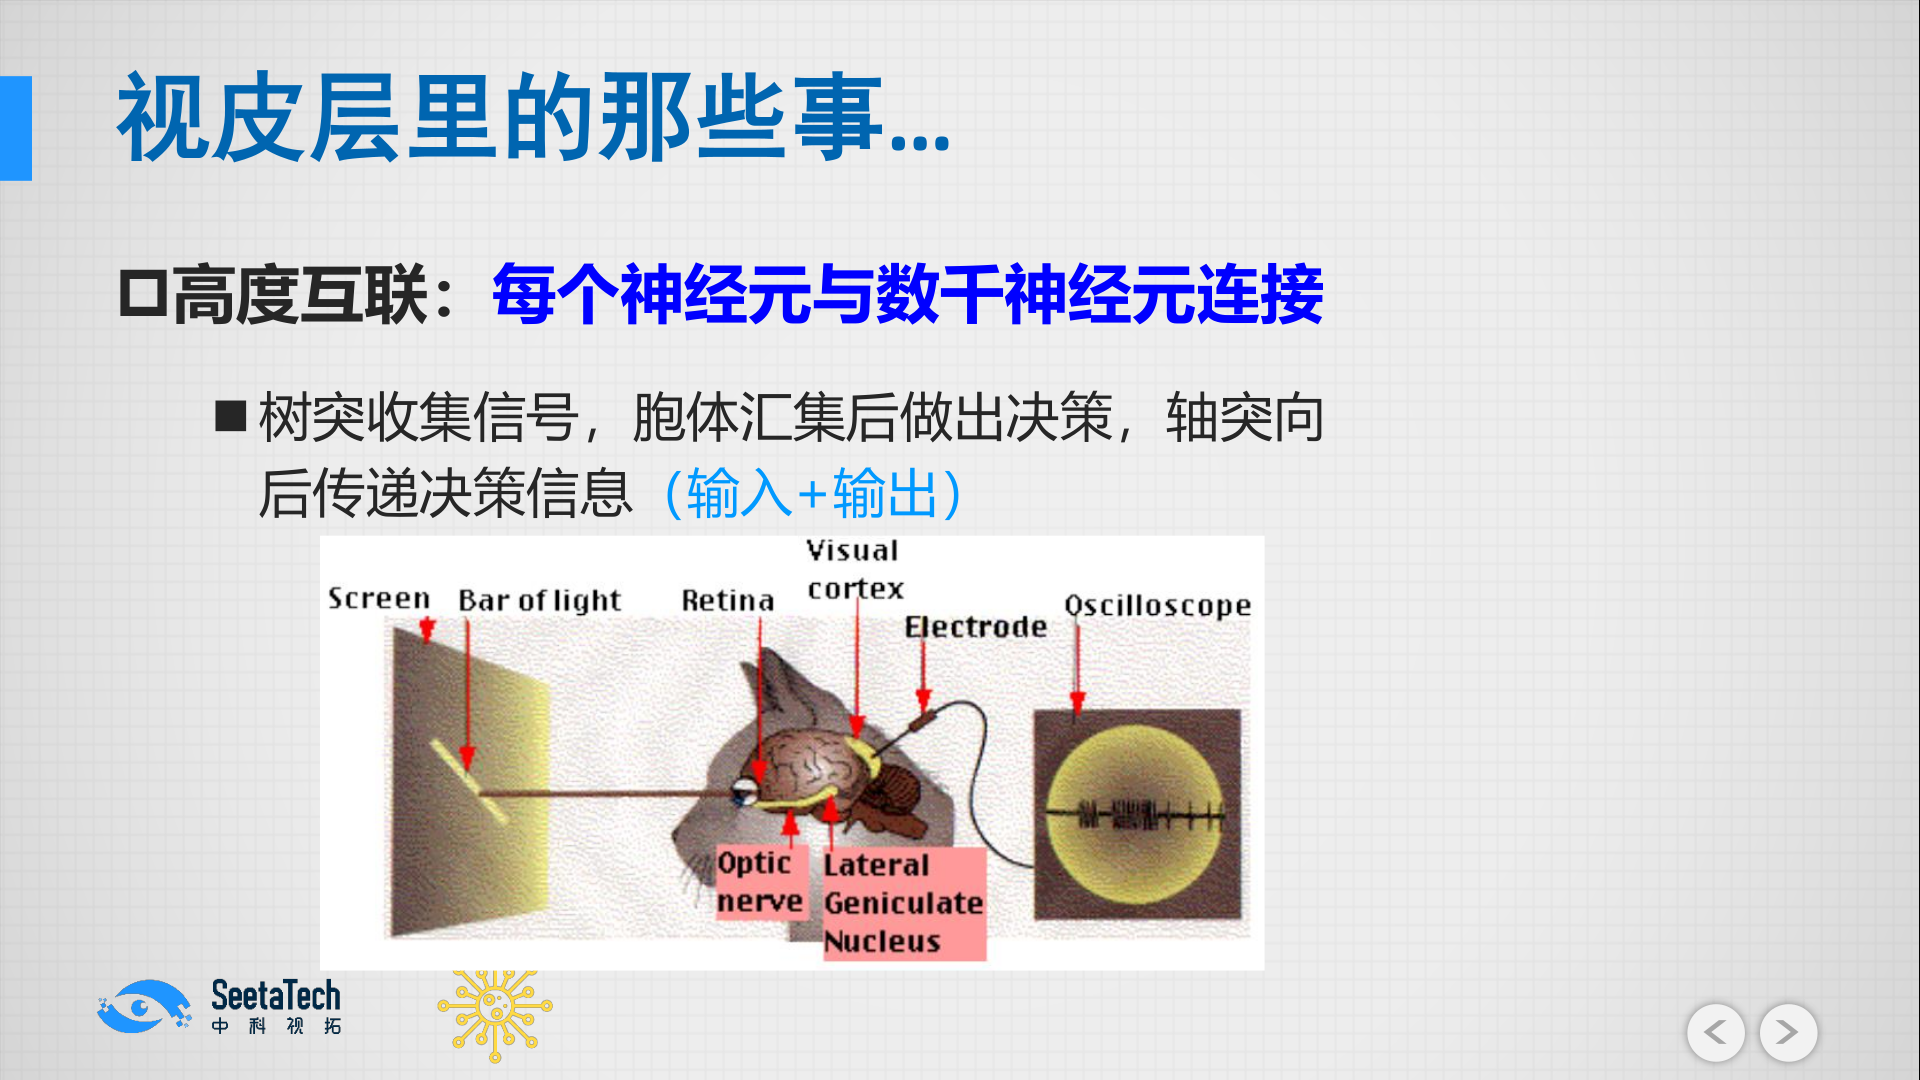
\includegraphics[width=6cm]{experiment.png}
\caption{The experiment}
\label{experiment}
\end{minipage}
\hfill
\begin{minipage}[t]{0.45\linewidth}
\centering
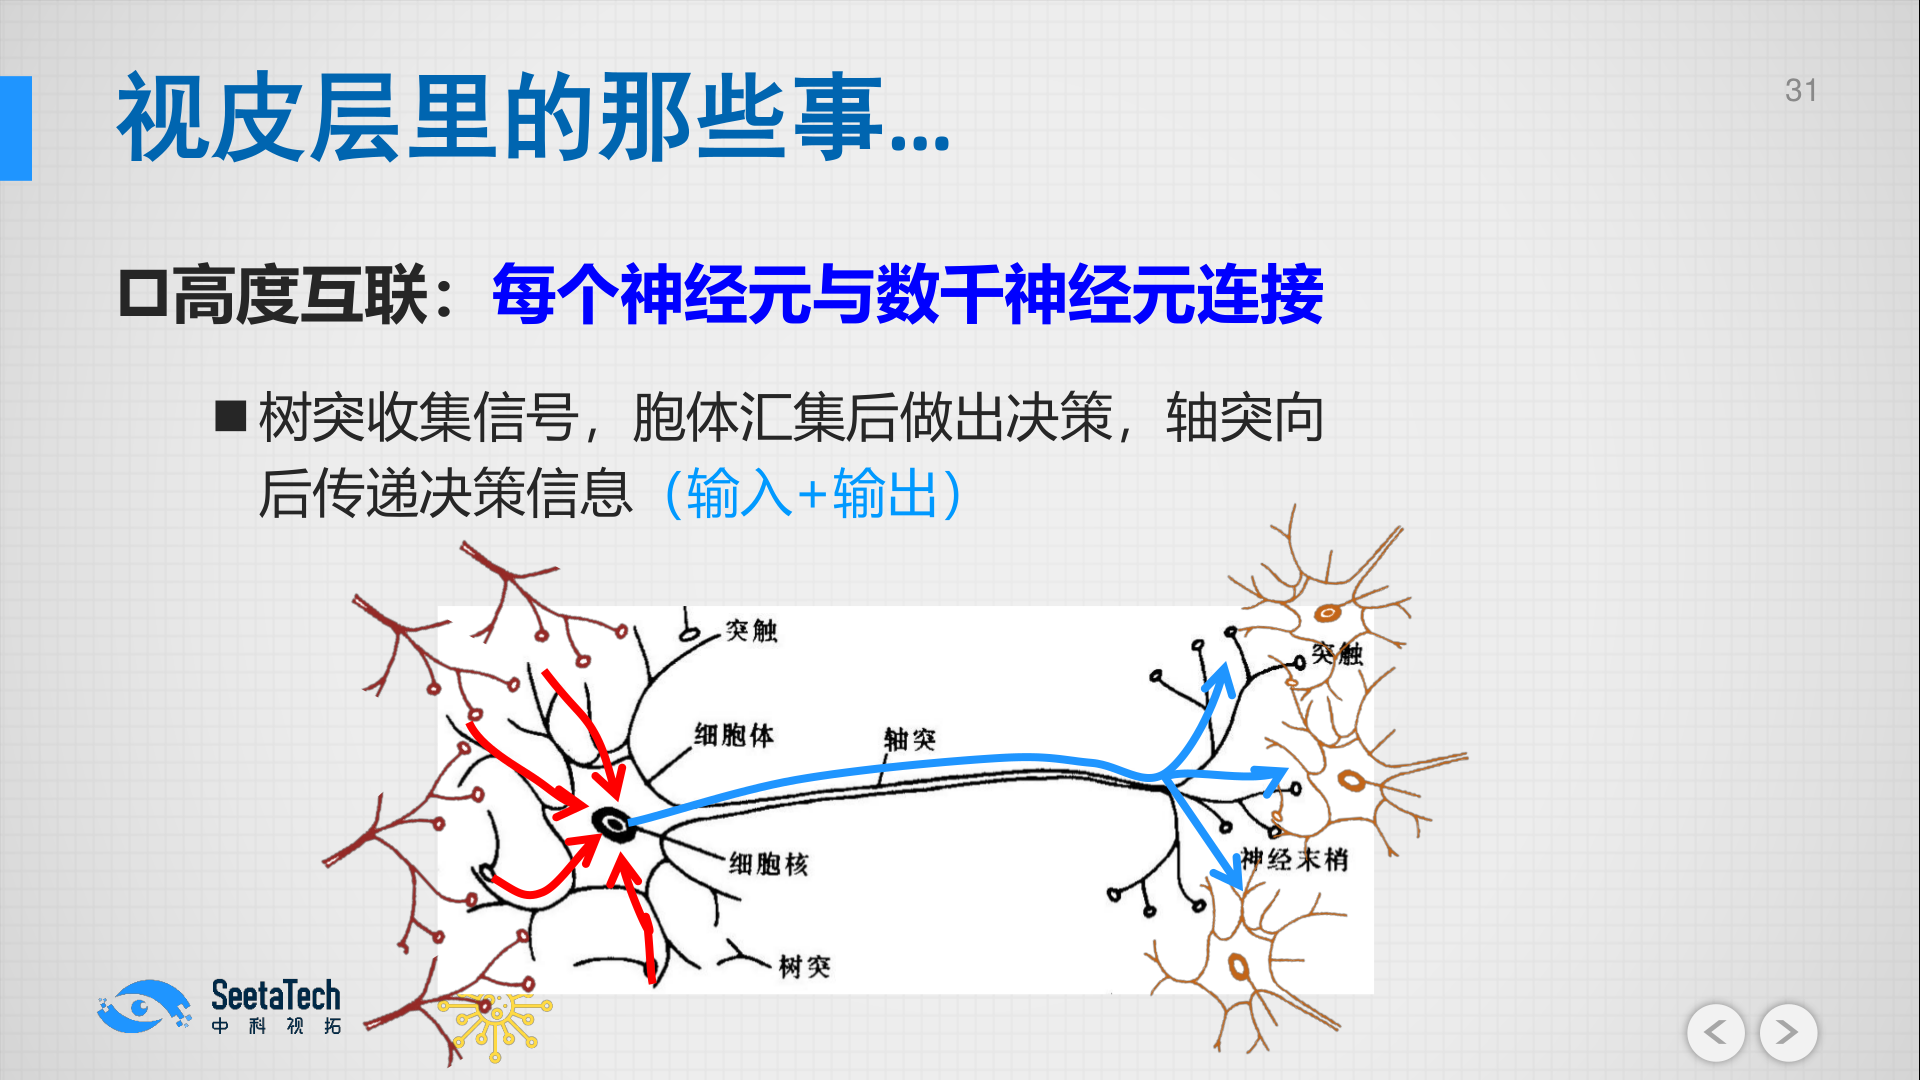
\includegraphics[width=6cm]{nerve_cells.png}
\caption{How nerve cells work}
\label{nervecells}
\end{minipage}

\end{figure}

\section{How can we imitate our brains}
In Deeplearning, every neuron represent a function which count the prossibility of a specific incident happening and they transmit the results to the next neuron which is used to count a more complex prossibility. By repeat the step above we can judge what we want precisely.

\begin{figure}[htbp]

\begin{minipage}[t]{0.3\linewidth}
\centering
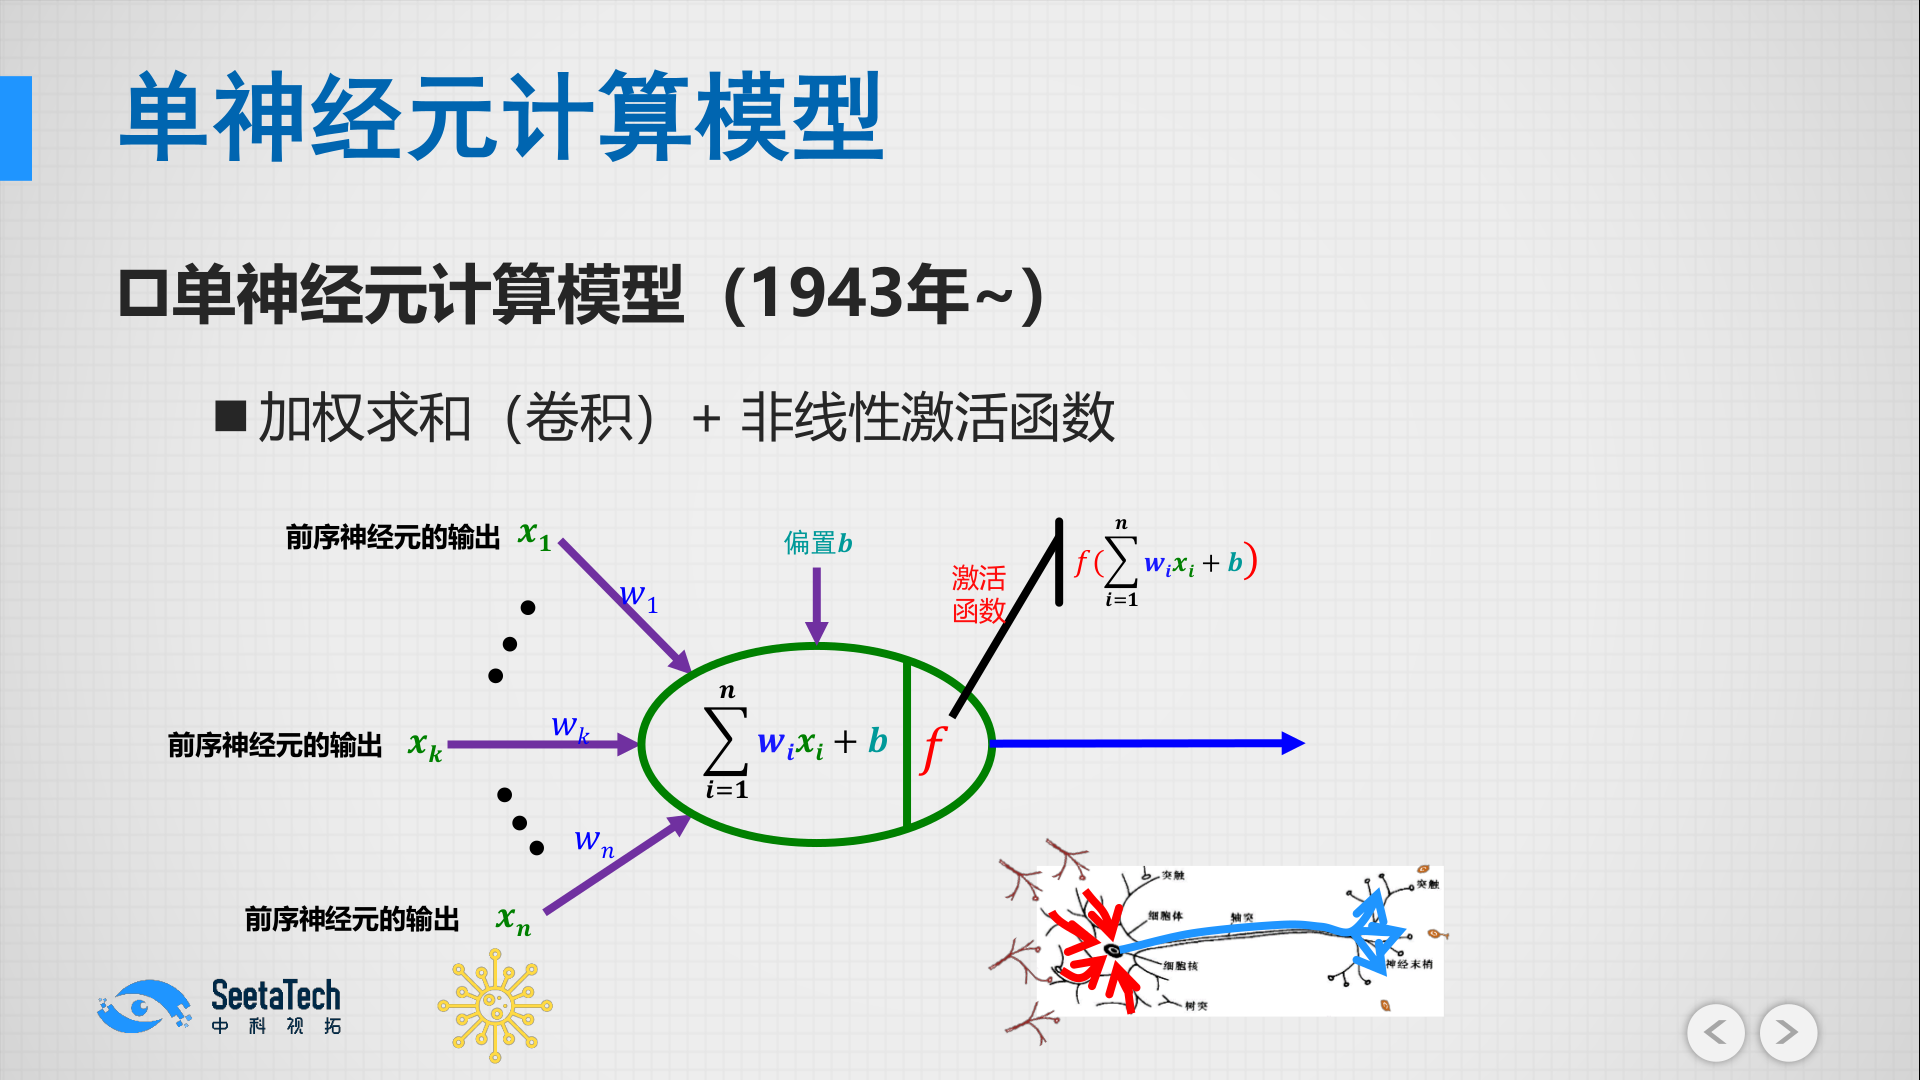
\includegraphics[width=4cm]{model.png}
\caption{Model}
\label{model}
\end{minipage}
\hfill
\begin{minipage}[t]{0.3\linewidth}
\centering
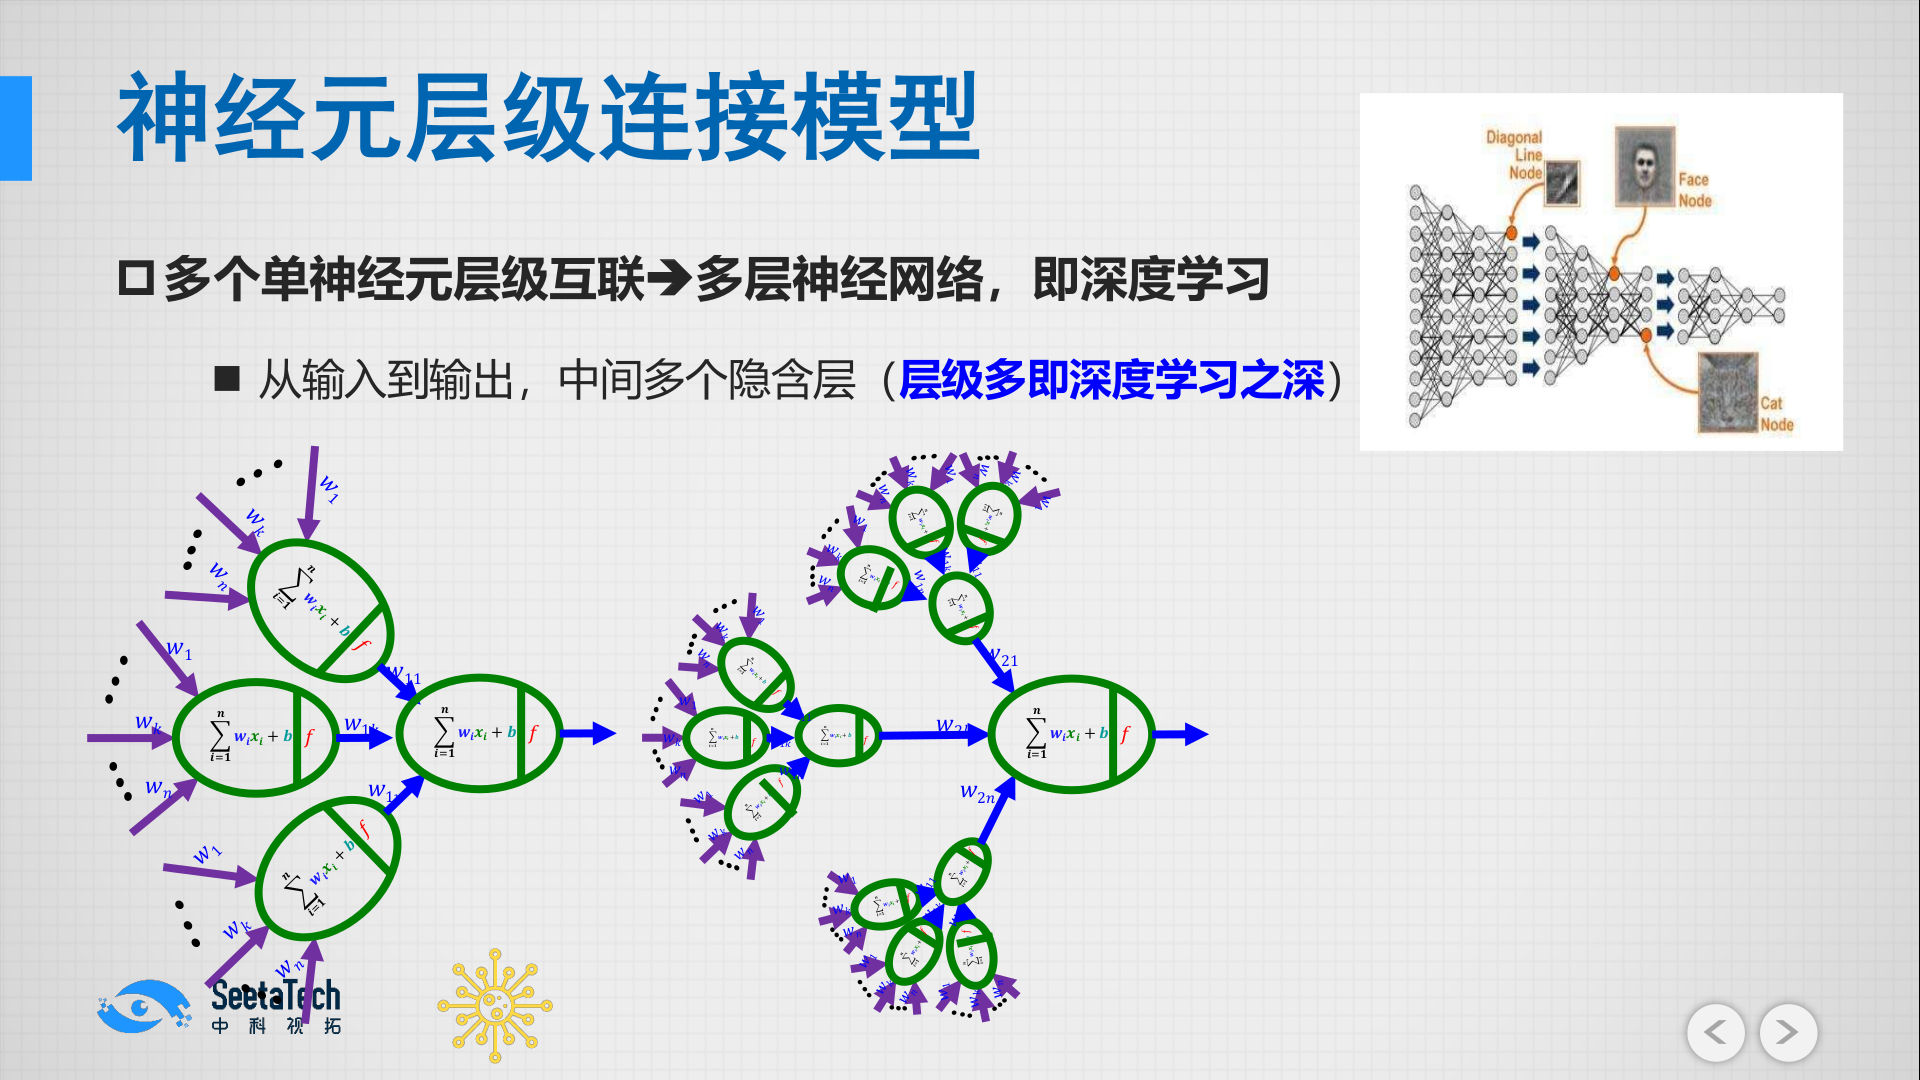
\includegraphics[width=4cm]{neural_net_work.png}
\caption{Neural net work}
\label{neuralnetwork}
\end{minipage}
\hfill
\begin{minipage}[t]{0.3\linewidth}
\centering
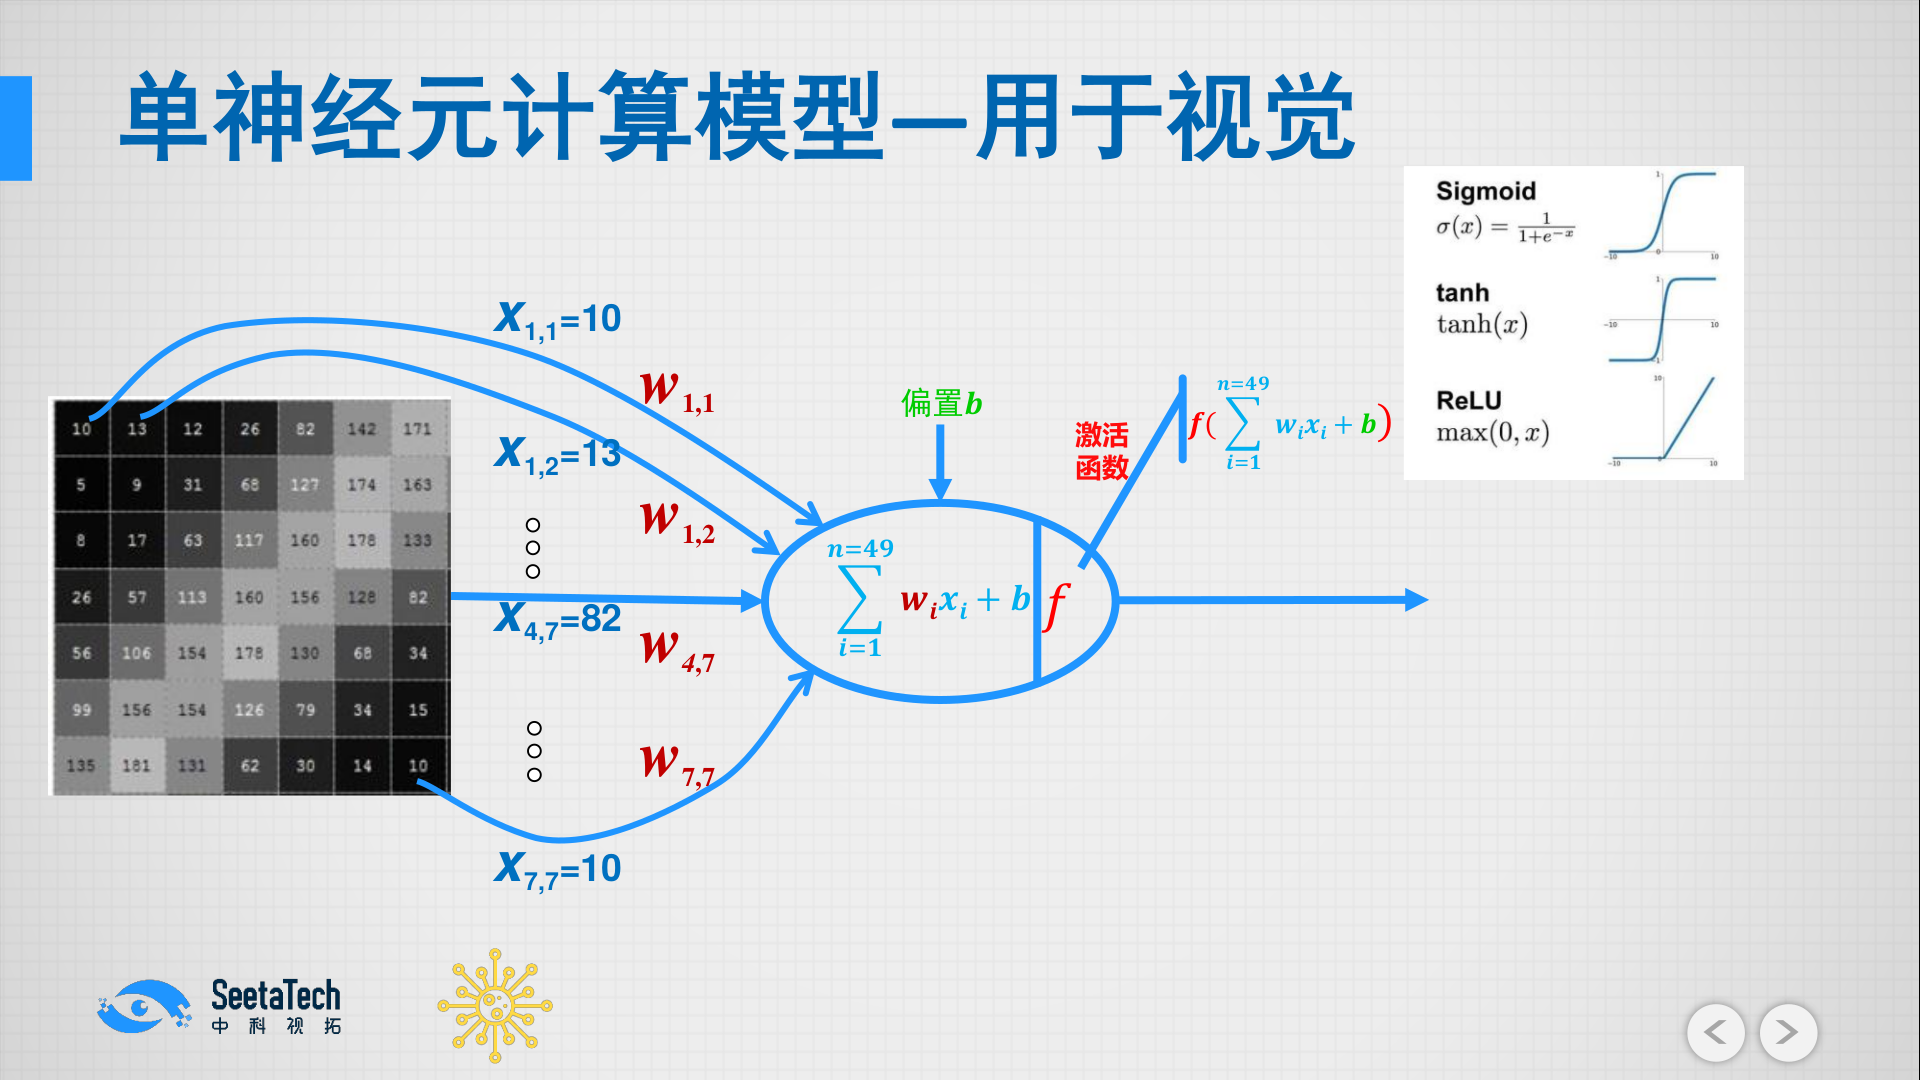
\includegraphics[width=4cm]{vision.png}
\caption{Applications in the vision field}
\label{vision}
\end{minipage}

\end{figure}

\addcontentsline{toc}{section}{Learning summary}
\section*{Learning summary}
This week I spend a lot of in configuring complier and studying python grammar. Now I can understand a little more about the codes in videos and homework. And videos from SeetaTech also helps a lot. I'll continue to watch it.\par
In this course, Practical aspects of DeepLearning, the knowledges points are much more mathematical, which makes it harder for me to understand. I'll spend more time in practicing instead of watching the next week so that I can grasp the technology expertly.
\end{document}
